\section{Introduction}
Autonomous vehicles need to navigate in dynamic environments in a safe and comfortable manner.  
This requires predicting the future motions of other agents to understand how the 
scene will evolve. 
However, depending on each agent's intention (e.g. turning, lane-changing), the agents' future motions can involve complicated maneuvers such as yielding, nudging, and acceleration.
Even worse, those intentions are not known a priori by the ego-robot, and agents may also change their minds based on behaviors of nearby agents. 
Therefore, even with access to the ground-truth trajectory histories of the agents,
forecasting their motions is very challenging and is an unsolved problem.

By leveraging deep learning, the motion forecasting community has been making steady progress. 
Most state-of-the-art models share a similar design principle: using a single feature
vector to characterize all the information related to an actor as shown in Fig.~\ref{fig:teaser}, left.
They typically first encode for each actor
its past motions and the surrounding context (\eg, map information) into a feature
vector, which is computed either by feeding a 2D rasterization to a
convolutional neural network (CNN)
\cite{nmp,dsd,precog,chauffeurnet,covernet,intentnet}, or directly using a
recurrent neural network (RNN)
\cite{matf,mfp,vectornet,tnt,sociallstm}.
Next, they exchange the information among actors to model interactions, \eg, via a fully-connected
graph neural network (GNN)
\cite{v2vnet,spagnn,precog,mfp,vectornet} or an attention
mechanism \cite{interacttransformer,sophie,socialatt,carnet,mercat2020multi}. 
Finally, they predict future motions per actor from its feature vector
% via a regression header \cite{nmp,lgn,mfp,precog,pnpnet,attnmp}.
via a regression header \cite{nmp,lgn,mfp,precog,pnpnet}.


\begin{figure}[t]
\begin{center}
  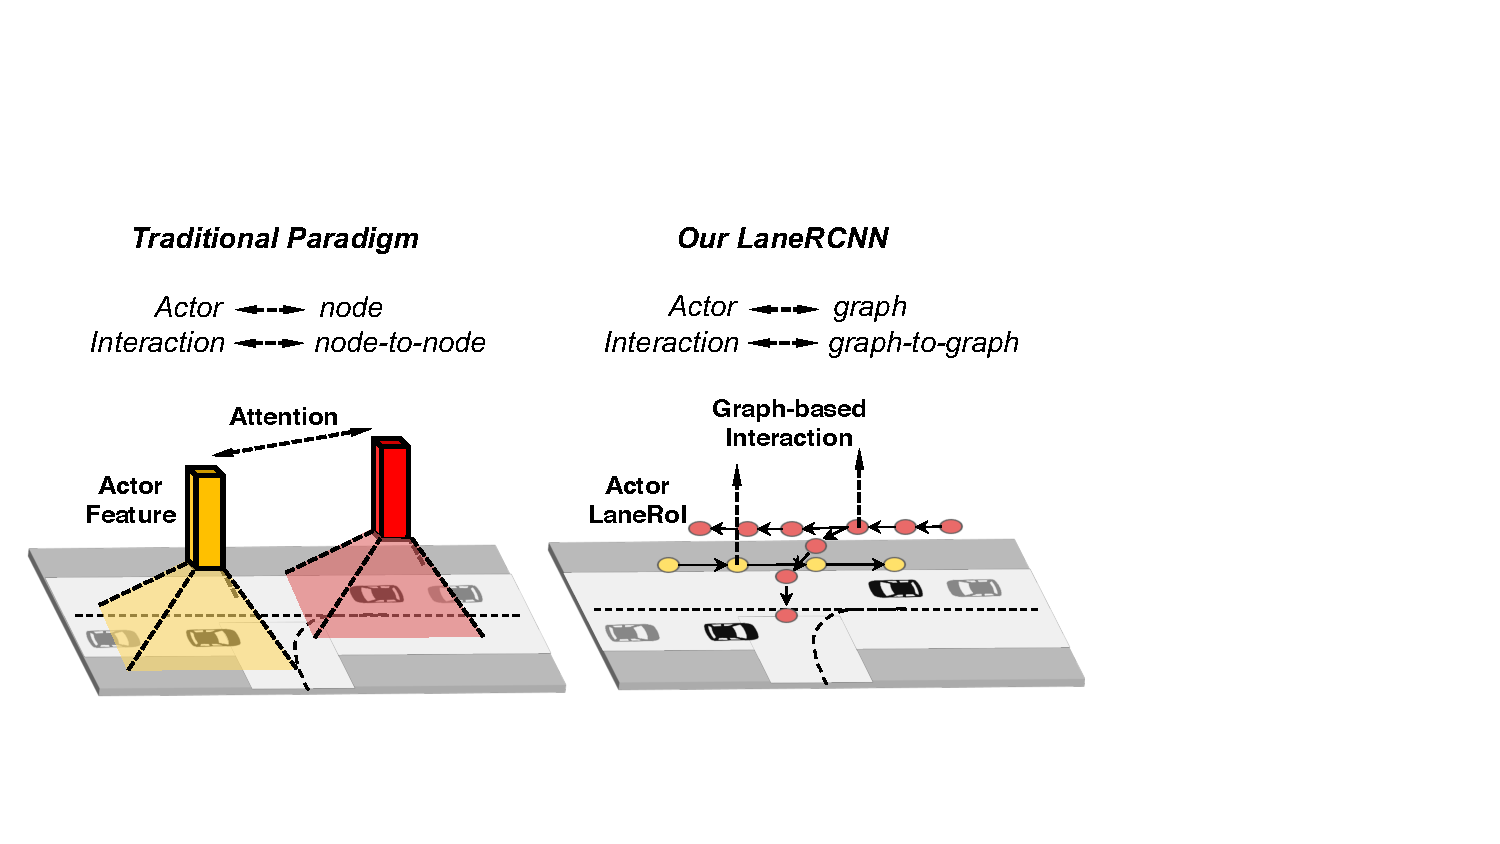
\includegraphics[height=3.4cm]{figures/teaser.pdf}
\end{center}
\vspace{-0.2cm}
\caption{Popular motion forecasting methods encode actor and its context
information into a feature vector, and treat it as a node in an interaction graph.
In contrast, we propose a graph-based
representation \ROI per actor, which is structured and expressive. Based on
it, we model interactions and forecast motion in a map topology aware manner.}
\label{fig:teaser}
\vspace{-0.2cm}
\end{figure}



\begin{figure*}[t]
\vspace{-0.2cm}
\begin{center}
  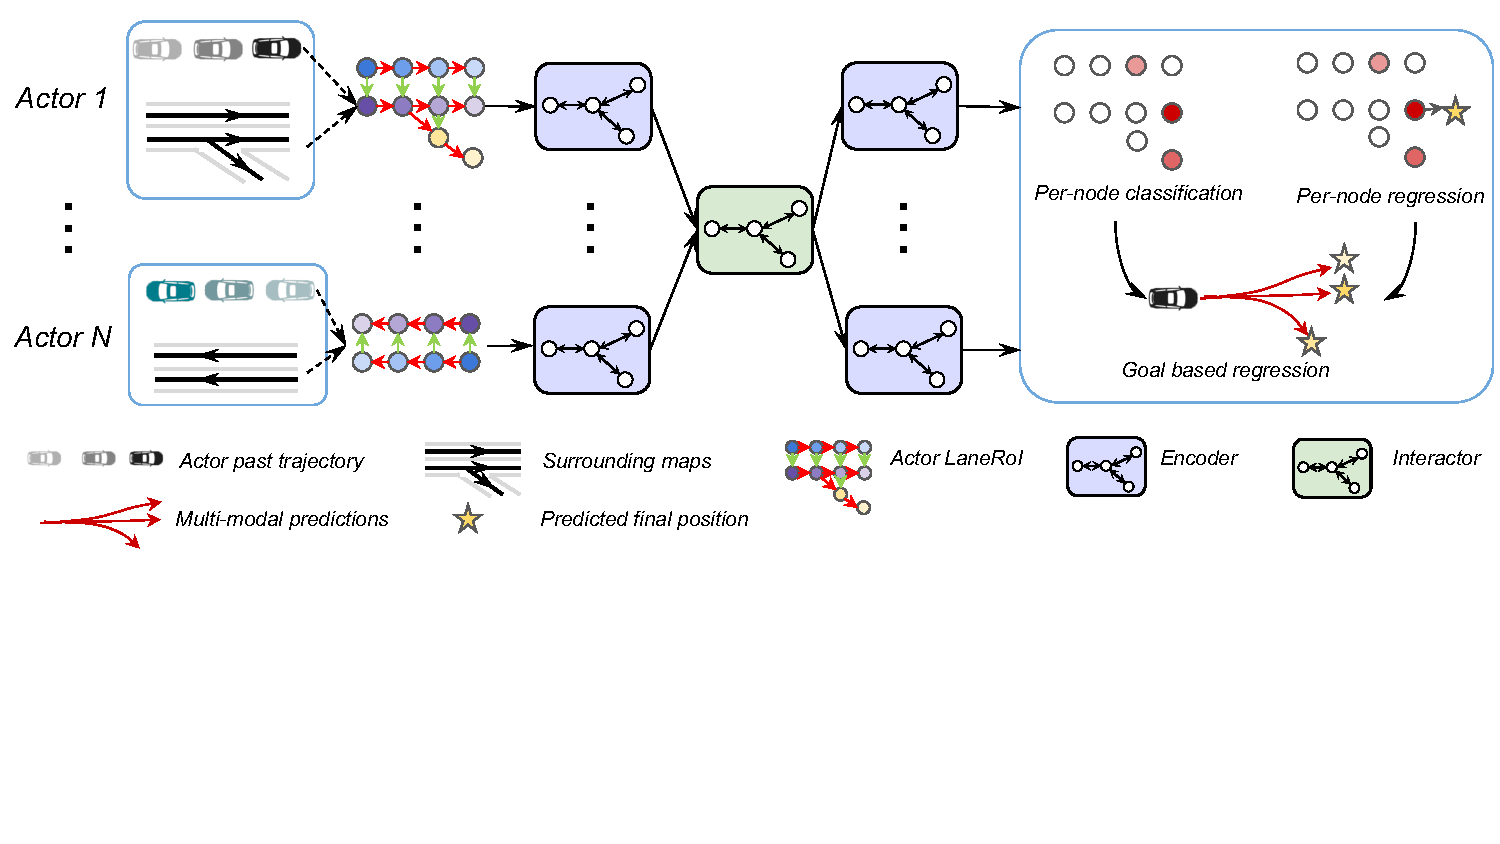
\includegraphics[height=5.8cm]{figures/lanercnn.pdf}
\end{center}
\vspace{-0.3cm}
\caption{Overview of LaneRCNN. It first
encodes each actor with our proposed \ROI representation, processes
each \ROI with an encoder, and then models interactions among actors with a
graph-based interactor. Finally, LaneRCNN predicts final positions of actors in
a fully-convolutional manner, and then decodes full trajectories based on these
positions.}
\vspace{-0.2cm}
\label{fig:lanercnn}
\end{figure*}

Although such a paradigm has shown competitive results, it has three main shortcomings:
1) Representing the context information of large regions of space, such as fast
moving actors traversing possibly a hundred meters within five seconds, with a
single vector is difficult, as we will show in our experiments.
2) Building a fully-connected interaction graph among actors ignores important map
structures~\cite{lgn}. For example, an unprotected left turn vehicle should yield to oncoming traffic, while two
spatially nearby vehicles driving on opposite lanes barely interact with each other.
3) The regression header does not explicitly leverage the lane information, which could provide a good inductive bias for accurate predictions. 
As a consequence, regression-based
predictors sometimes forecast \textit{shooting-out-of-road} trajectories, which
are unrealistic. 






In this paper, we propose a graph-centric motion forecasting model, \ie, LaneRCNN, 
to address the aforementioned issues. 
We represent an actor and its context 
in a distributed and map-aware manner by 
constructing an actor-specific graph, called Lane-graph Region-of-Interest (\textit{LaneRoI}), along with node 
embeddings that encode the past motion and map semantics. 
In particular, we construct  \textit{LaneRoI} following the topology 
of lanes that are relevant to this actor, where nodes on this graph correspond
to small spatial regions along these lanes, and edges represent the topological and spatial relations among regions. 
Compared to using a single vector to encode all the information of a large region, our \textit{LaneRoI} naturally
preserves the map structure and captures the more fine-grained information, 
as each node embedding only needs to represent the local context within a small
region. 
To model interactions, we embed the \textit{LaneRoI}s of all actors to
a global lane graph  and then propagate the information over this global graph.
Since the \textit{LaneRoI}'s of interacting actors are highly relevant, those actors will
share overlapping regions on the global graph, thus having more frequent
communications during the information propagation compared to 
irrelevant actors. 
Importantly, this process neither requires any heuristics nor makes any oversimplified
assumptions while learning interactions conditioned on maps. 
We then predict future motions on each
\textit{LaneRoI} in a \emph{fully-convolutional} manner, such that small regions along
lanes (nodes in \textit{LaneRoI}) can serve as anchors and provide good priors
. We demonstrate the effectiveness of our method on the
large-scale Argoverse motion forecasting benchmark \cite{argoverse}, and
achieve state-of-the-art performance evaluated by the official ranking metric.
